\documentclass[conference]{IEEEtran}

\ifCLASSOPTIONcompsoc
\usepackage[nocompress]{cite}
\else
\usepackage{cite}
\fi

\usepackage{flushend}

\usepackage[pdftex]{graphicx}
\graphicspath{{./pdf/}}
\DeclareGraphicsExtensions{.pdf}

\ifCLASSINFOpdf
% \usepackage[pdftex]{graphicx}
% declare the path(s) where your graphic files are
% \graphicspath{{../pdf/}{../jpeg/}}
% and their extensions so you won't have to specify these with
% every instance of \includegraphics
%\DeclareGraphicsExtensions{.pdf,.jpeg,.png}
\else
% or other class option (dvipsone, dvipdf, if not using dvips). graphicx
% will default to the driver specified in the system graphics.cfg if no
% driver is specified.
% \usepackage[dvips]{graphicx}
% declare the path(s) where your graphic files are
% \graphicspath{{../eps/}}
% and their extensions so you won't have to specify these with
% every instance of \includegraphics
% \DeclareGraphicsExtensions{.eps}
\fi
% graphicx was written by David Carlisle and Sebastian Rahtz. It is
% required if you want graphics, photos, etc. graphicx.sty is already
% installed on most LaTeX systems. The latest version and documentation
% can be obtained at: 
% http://www.ctan.org/pkg/graphicx
% Another good source of documentation is "Using Imported Graphics in
% LaTeX2e" by Keith Reckdahl which can be found at:
% http://www.ctan.org/pkg/epslatex
% 
% latex, and pdflatex in dvi mode, support graphics in encapsulated
% postscript (.eps) format. pdflatex in pdf mode supports graphics
% in .pdf, .jpeg, .png and .mps (metapost) formats. Users should ensure
% that all non-photo figures use a vector format (.eps, .pdf, .mps) and
% not a bitmapped formats (.jpeg, .png). The IEEE frowns on bitmapped formats
% which can result in "jaggedy"/blurry rendering of lines and letters as
% well as large increases in file sizes.
% 
% You can find documentation about the pdfTeX application at:
% http://www.tug.org/applications/pdftex


% *** MATH PACKAGES ***
\usepackage{amsmath}
\interdisplaylinepenalty=2500

% *** ALIGNMENT PACKAGES ***
% 
% \usepackage{array}
% Frank Mittelbach's and David Carlisle's array.sty patches and improves
% the standard LaTeX2e array and tabular environments to provide better
% appearance and additional user controls. As the default LaTeX2e table
% generation code is lacking to the point of almost being broken with
% respect to the quality of the end results, all users are strongly
% advised to use an enhanced (at the very least that provided by array.sty)
% set of table tools. array.sty is already installed on most systems. The
% latest version and documentation can be obtained at:
% http://www.ctan.org/pkg/array

\hyphenation{op-tical net-works semi-conduc-tor}

\begin{document}
\title{Using an Intuitionistic Fuzzy Inference System for
Classification Problems}

\author{\IEEEauthorblockN{Amaury Hernandez-Aguila, Mario
    Garcia-Valdez, Oscar Castillo}
  \IEEEauthorblockA{Tijuana Institute of Technology\\
    Division of Graduate Studies and Graduates\\
    Tijuana, Mexico\\
    Email: \{amherag,mario,ocastillo\}@tectijuana.edu.mx}}

\maketitle

\begin{abstract}

\end{abstract}

\IEEEpeerreviewmaketitle

\section{Introduction}
\label{introduction}

\section{Related Work}
\label{related-work}

% intuitionistic fuzzy set
\begin{equation}
  \label{ifs-implication}
  \begin{aligned}
  A \implies B = & \{ \langle x, max(\nu_{A} (x), \mu_{B}(x)),\\
  &\quad min(\mu_{A} (x), \nu_{B} (x)) \rangle | x \in E \}
\end{aligned}
\end{equation}

\begin{equation}
  \label{linear-combination}
  IFS = (1-\pi)FS_{\mu} + \pi FS_{v}
\end{equation}

\section{Preliminaries}
\label{preliminaries}

% intuitionistic fuzzy set
\begin{equation}
  \label{ifs-definition}
  A^{*} = \{\langle x, \mu _{A} (x), \nu _{A} (x) \rangle | x \in E\}
\end{equation}

% intuitionistic interval
\begin{equation}
  \label{intuitionistic-interval}
  0 \leq \mu_{A}(x) + \nu_{A}(x) \leq 1
\end{equation}

% every ordinary fuzzy set has the form
\begin{equation}
  \label{ifs-form}
  \{ \langle x, \mu_{A}(x), 1 - \mu_{A}(x) \rangle | x \in E \}
\end{equation}

% if
\begin{equation}
  \label{fs-as-ifs-if}
  \pi_{A}(x) = 1 - \mu_{A}(x) - \nu_{A}(x)
\end{equation}

\section{Proposed Method}
\label{proposed-method}

\begin{figure}[!t]
  \centering
  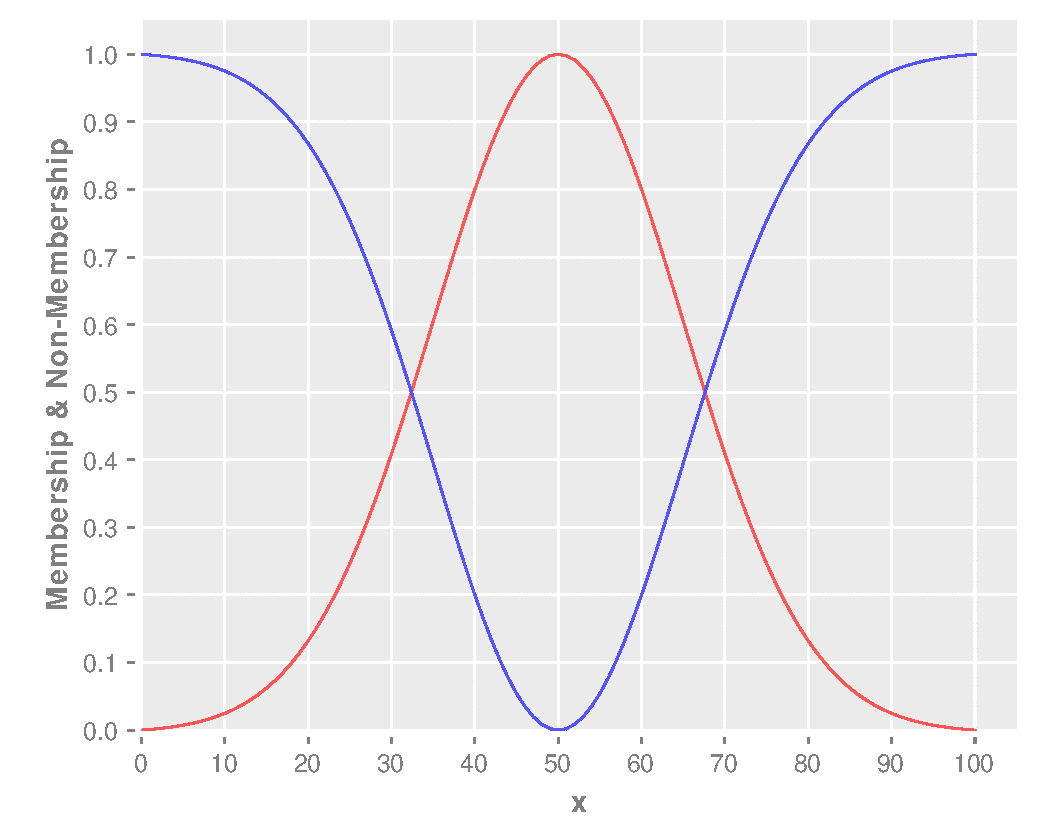
\includegraphics[width=3.0in]{fs-as-ifs}
  \caption{Traditional Fuzzy Set Represented as an Intuitionistic Fuzzy Set}
  \label{fs-as-ifs}
\end{figure}

\begin{figure}[!t]
  \centering
  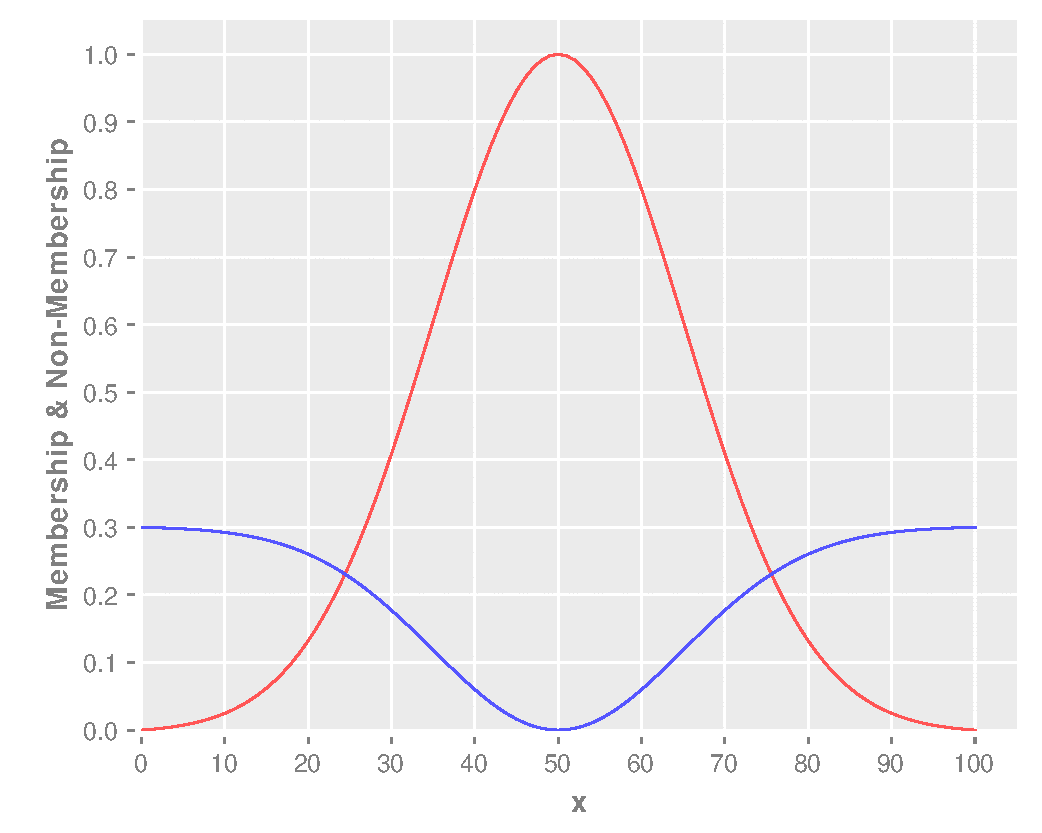
\includegraphics[width=3.0in]{ifs}
  \caption{An Example of an Intuitionistic Fuzzy Set - Same Mean and SD}
  \label{ifs}
\end{figure}

\begin{figure}[!t]
  \centering
  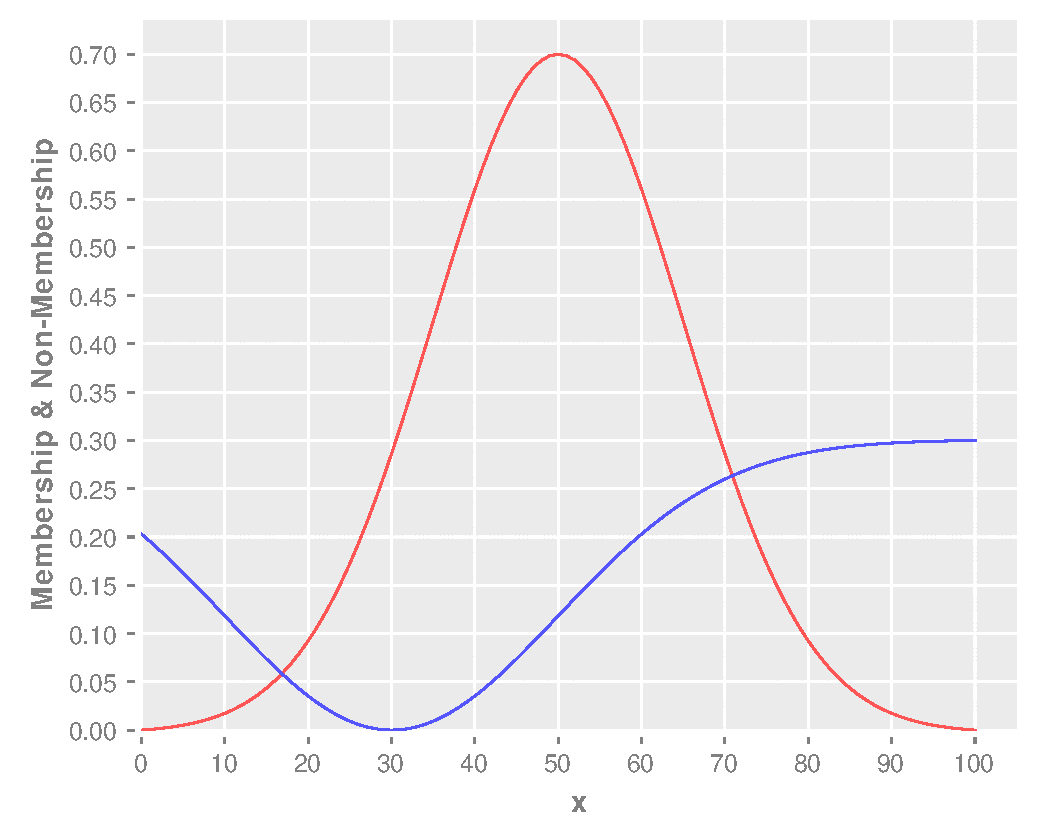
\includegraphics[width=3.0in]{ifs-diff-mu-sd}
  \caption{An Example of an Intuitionistic Fuzzy Set - Different Mean
    and SD}
  \label{ifs-diff-mu-sd}
\end{figure}

\begin{figure}[!t]
  \centering
  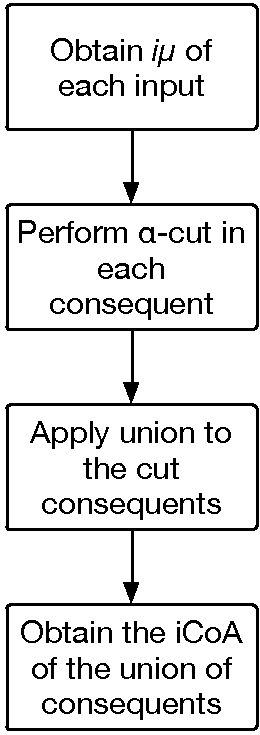
\includegraphics[height=2.5in]{proposed-method-flow-chart}
  \caption{Proposed Method Flow Chart}
  \label{flow-chart}
\end{figure}

% i-membership
\begin{equation}
  \label{imembership}
  i\mu_{A}(x) = (\nu_{A}(x) + \mu_{A}(x))\mu_{A}(x)
\end{equation}

\begin{figure}[!t]
  \centering
  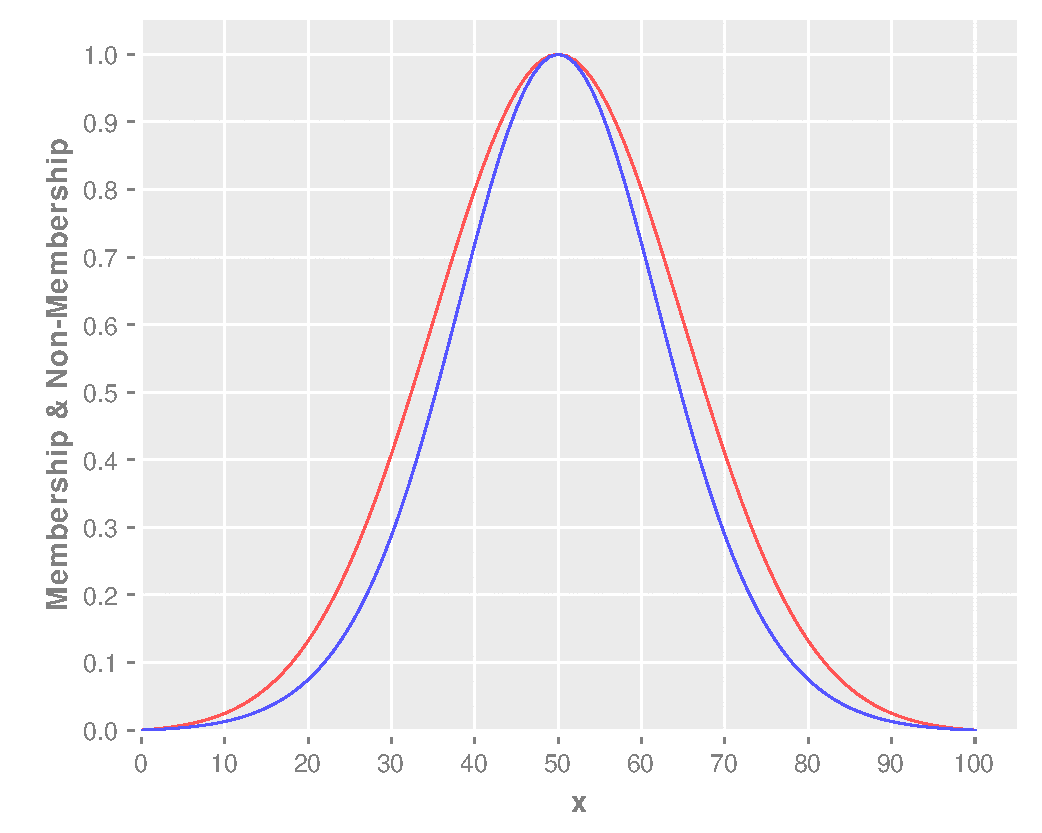
\includegraphics[width=3.0in]{if-membership}
  \caption{Comparison of $\mu(x)$ Against $i\mu(x)$}
  \label{if-membership}
\end{figure}

\begin{figure}[!t]
  \centering
  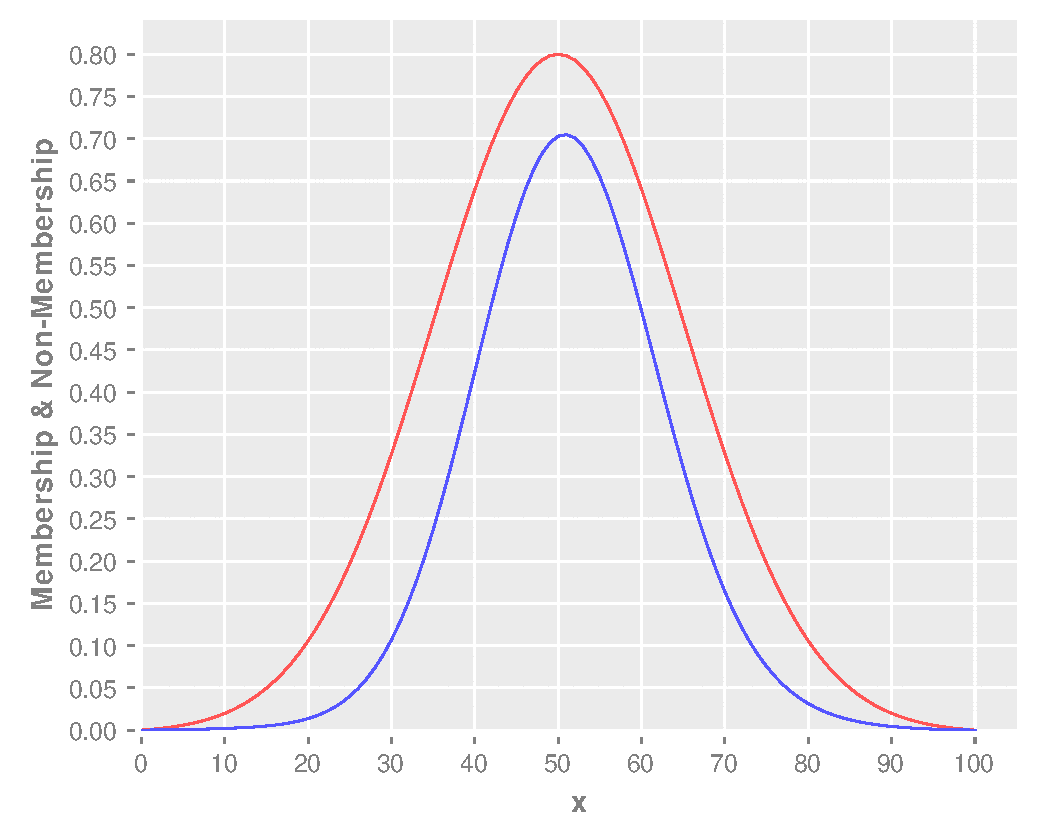
\includegraphics[width=3.0in]{if-membership-drastic}
  \caption{Comparison of $\mu(x)$ Against $i\mu(x)$ With More Indeterminism}
  \label{if-membership-drastic}
\end{figure}

\begin{equation}
  \label{alpha-cut}
  \alpha(\mu (x),\mu_{\alpha}) =
  \begin{cases}
    \mu (x), & \text{if}\ \mu (x) \leq \mu_{alpha}  \\
    \mu_{\alpha}, & \text{otherwise}
  \end{cases}
\end{equation}

\begin{equation}
  \label{nmf-alpha-cut}
  \alpha_{NMF}(\nu (x),\mu_{\alpha}) =
  \begin{cases}
    \nu (x), & \text{if}\ \nu (x) \geq \nu (\mu_{alpha})  \\
    \nu (\mu_{alpha}), & \text{otherwise}
  \end{cases}
\end{equation}

\begin{figure}[!t]
  \centering
  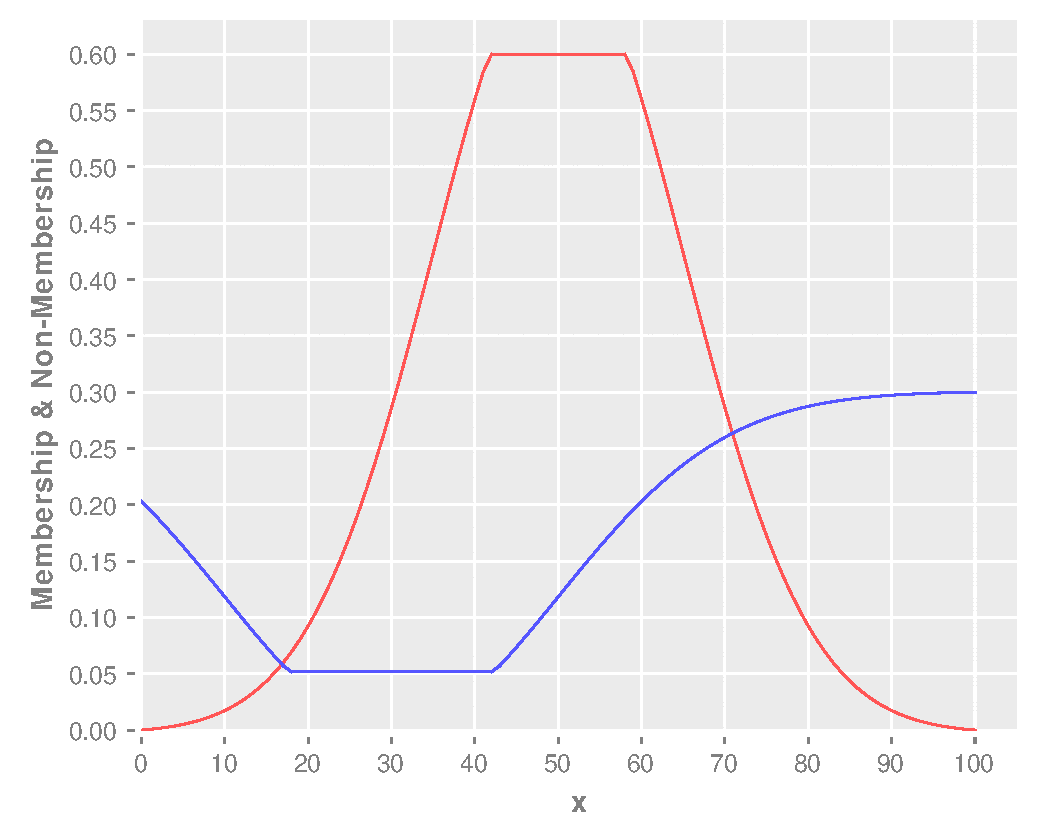
\includegraphics[width=3.0in]{alpha-cut}
  \caption{$\alpha$-cut of an Intuitionistic Fuzzy Set}
  \label{alpha-cut-example}
\end{figure}

\begin{equation}
  \label{union-operator}
  \begin{aligned}
    A \cup B  = &\{ \langle x, max(\mu_{A} (x), \mu_{B} (x)),\\
    &\quad min(\nu_{A} (x), \nu_{B} (x)) \rangle | x \in E \}
\end{aligned}
\end{equation}

\begin{figure}[!t]
  \centering
  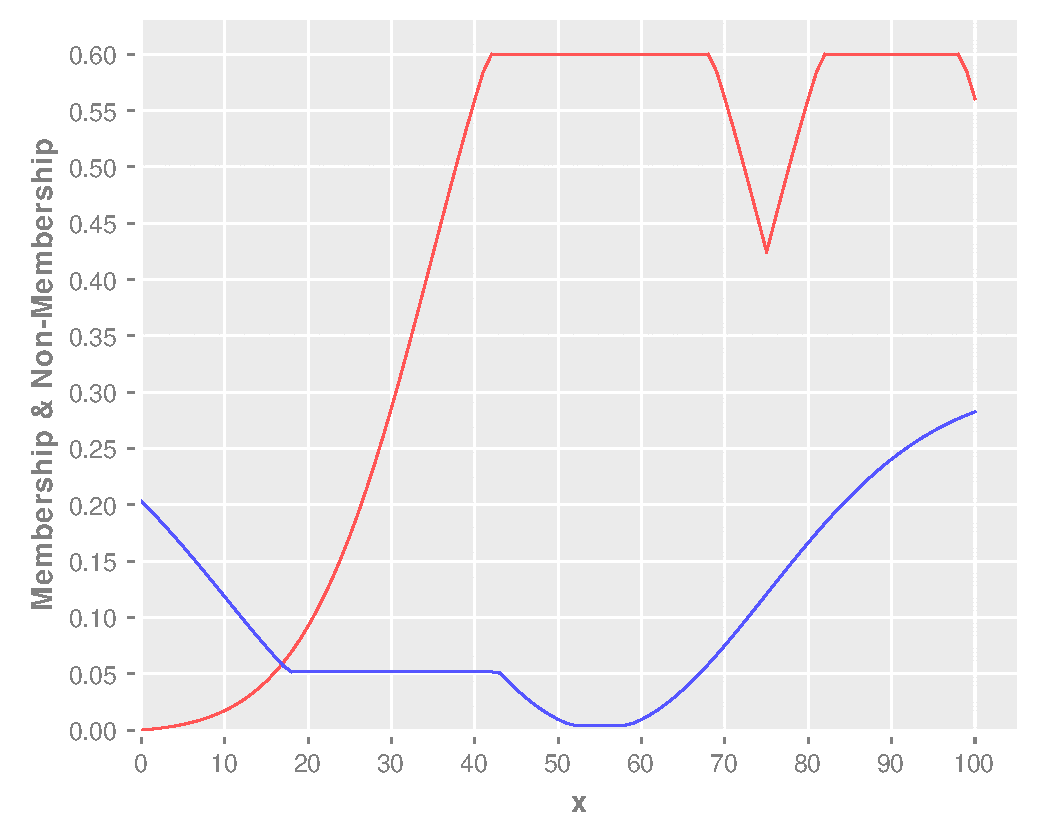
\includegraphics[width=3.0in]{ifs-union}
  \caption{Union of Three $\alpha$-cut Intuitionistic Fuzzy Sets}
  \label{ifs-union}
\end{figure}

% CoA
\begin{equation}
  \label{center-of-area}
  A_{CoA} = \dfrac{\sum_{i=1}^{N} \mu(x_{i})
    x_{i}}{\sum_{i=1}^{N} \mu(x_{i})}
\end{equation}

%iCoA
\begin{equation}
  \label{if-coa}
  A_{iCoA} = \dfrac{\sum_{i=1}^{N} (\mu(x_{i}) + \nu(x_{i})) \mu(x_{i})
    x_{i}}{\sum_{i=1}^{N} (\mu(x_{i}) + \nu(x_{i})) \mu(x_{i})}
\end{equation}

%iCoA contracted
\begin{equation}
  \label{if-coa-simplified}
  A_{iCoA} = \dfrac{\sum_{i=1}^{N} i\mu_{A}(x) x_{i}}{\sum_{i=1}^{N}
    i\mu_{A}(x)}
\end{equation}

\begin{figure}[!t]
  \centering
  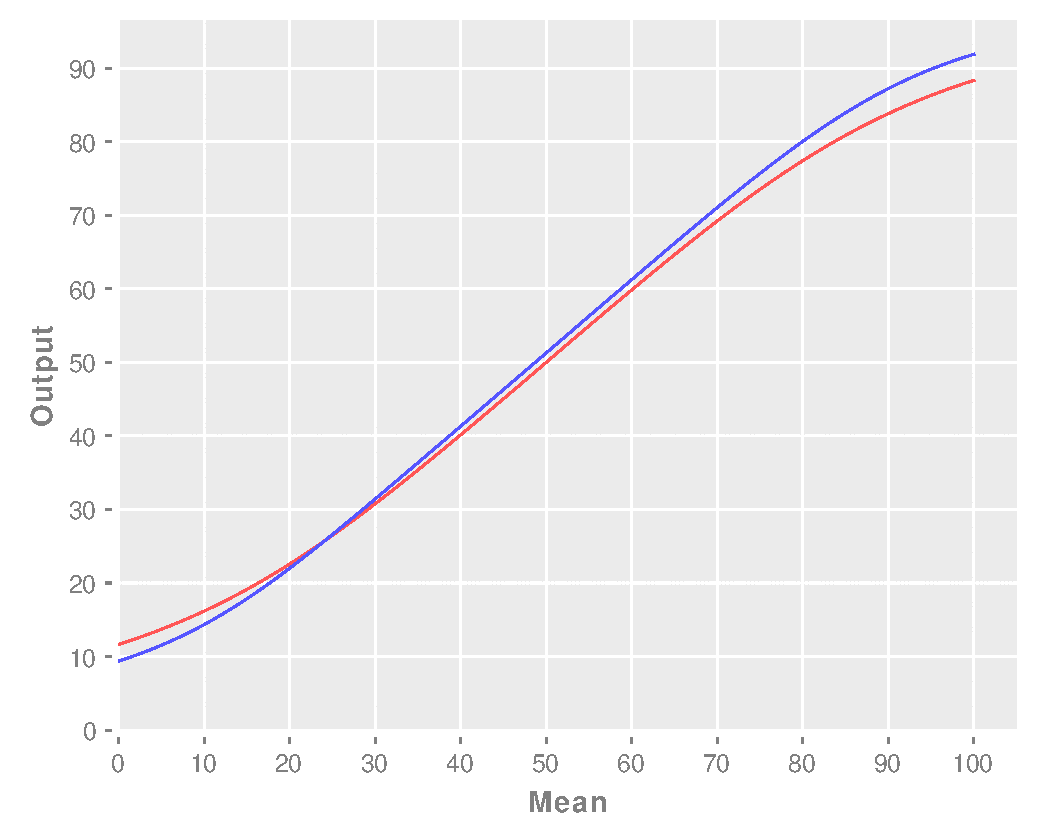
\includegraphics[width=3.0in]{if-coa-vs-coa}
  \caption{Comparison of $CoA_{A_{i}}$ Against $iCoA_{A_{i}}$}
  \label{if-coa-vs-coa}
\end{figure}

\section{Experiments}
\label{experiments}

\begin{enumerate}
  \item if $t_{0}$ is $A_{1}$ then $p_{t+1}$ is $C_{1}$
  \item if $t_{-6}$ is $A_{2}$ then $p_{t+1}$ is $C_{2}$
  \item if $t_{-12}$ is $A_{3}$ then $p_{t+1}$ is $C_{3}$
  \item if $t_{-18}$ is $A_{4}$ then $p_{t+1}$ is $C_{4}$
\end{enumerate}

\begin{equation}
  \label{scaling}
  S(p) = 100 \frac{p - min(P)}{max(P) - min(P)}
\end{equation}

\section{Results}
\label{results}

\section{Conclusion}
\label{conclusion}

\section{Future Work}
\label{future-work}

\bibliographystyle{IEEEtran}
\bibliography{paper}

\end{document}
